\documentclass[12pt]{scrartcl}
\usepackage[sexy]{evan}
\usepackage{graphicx,amsmath,amssymb,amsthm,amsfonts,babel}
\usepackage{tikz, tkz-euclide}
\usepackage{lipsum}
\usepackage{setspace}
\graphicspath{ {./} }
\usetikzlibrary{calc,through,intersections}
\usepackage[paperwidth=16.5cm, paperheight=16.5cm,margin=0.8cm]{geometry}

\colorlet{EvanRed}{Red!50!Purple}

\newcommand{\siku}[4][.5cm]
	{
	\coordinate (tempa) at ($(#3)!#1!(#2)$);
	\coordinate (tempb) at ($(#3)!#1!(#4)$);
	\coordinate (tempc) at ($(tempa)!0.5!(tempb)$);%midpoint
	\draw[black] (tempa) -- ($(#3)!2!(tempc)$) -- (tempb);
	}
	\usetikzlibrary{calc,positioning,intersections}

\setstretch{1.5}

\usepackage{etoolbox}
\newcommand{\zerodisplayskips}{%
  \setlength{\abovedisplayskip}{5pt}%
  \setlength{\belowdisplayskip}{5pt}%
  \setlength{\abovedisplayshortskip}{5pt}%
  \setlength{\belowdisplayshortskip}{5pt}}
\appto{\normalsize}{\zerodisplayskips}
\appto{\small}{\zerodisplayskips}
\appto{\footnotesize}{\zerodisplayskips}
\setlength\parindent{10pt}

\title{"OSN Korea" 2023 Nomor 1}
\author{KMO Final Round 2023 Problem 1}
\date{}

\pagestyle{empty}

\begin{document}

\maketitle
\newpage

\section{Soal}
\subsection{Soal Asli dalam Bahasa Korea}
\begin{center}
    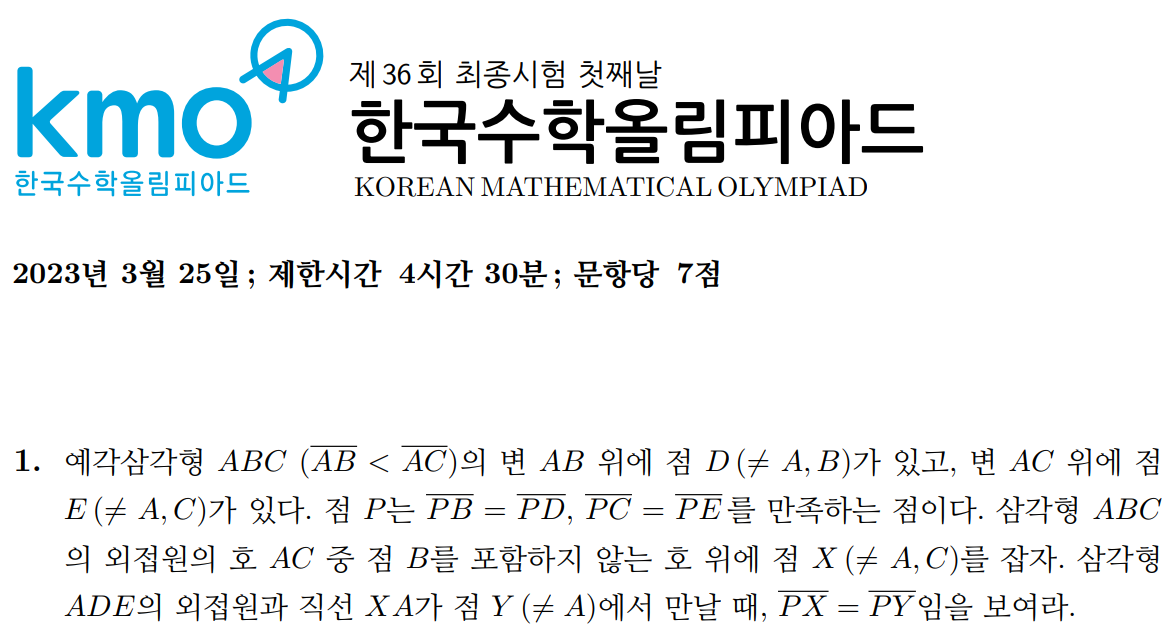
\includegraphics[scale=0.5]{KMO2023P1.png}
\end{center}
\subsection{Soal Terjemahan}
Pada sebuah segitiga $ABC ~(AB<AC)$, titik $D (\neq A, B)$ dan $E (\neq A, C)$ terletak pada sisi $AB$ dan $AC$ berturut-turut. Titik $P$ memenuhi $PB=PD$ dan $PC=PE$. Titik $X (\neq A, C)$ terletak pada busur $AC$ pada lingkaran luar segitiga $ABC$ yang tidak memuat $B$. Misalkan $Y (\neq A)$ adalah perpotongan lingkaran luar $ADE$ dan garis $XA$. Buktikan bahwa $PX=PY$.

\newpage
\section{Solusi}
    Misalkan garis $DE$ memotong garis $BC$ di $F$. Perhatikan bahwa $BCED$ merupakan \textit{complete quadrilateral} sehingga berdasarkan teorema Miquel, lingkaran $(ADE)$, $(BDF)$, $(CEF)$, dan $(ABC)$ bertemu di satu titik, misalkan di titik $G$. 

    \begin{center}
    \begin{asy}
        import olympiad;
        import geometry;
        size(300);
        pair A = dir(105);
        pair B = dir(210);
        pair C = dir(-30);
        pair D = B/4 + 3*A/4;
        pair E = 4*A/7 + 3*C/7;
        pair M = (B+D)/2;
        pair N = (C+E)/2;
        line MP = perpendicular(M, line(B,D));
        line NP = perpendicular(N, line(E,C));
        pair P = intersectionpoint(MP,NP);
        circle abc = circumcircle(triangle(A,B,C));
        pair X = dir(60);
        circle ade = circumcircle(triangle(A,D,E));
        pair AT[] = intersectionpoints(ade, line(A,X));
        pair Y = AT[0];
        pair AG[] = intersectionpoints(ade, abc);
        pair G = AG[1];
        circle amn = circumcircle(triangle(A,M,N));
        pair F = intersectionpoint(line(D,E),line(B,C));
        pair K = (X+Y)/2;
        dot("$A$", A, NW);
        dot("$B$", B, SW);
        dot("$C$", C, SE);
        dot("$D$", D, W);
        dot("$E$", E, 2.5*dir(0));
        dot("$M$", M, NW);
        dot("$N$", N, 2.5*dir(0));
        dot("$P$", P, S);
        dot("$X$", X, 2.5*dir(45));
        dot("$Y$", Y, SW);
        dot("$G$", G, NE);
        dot("$F$", F, NE);
        dot("$K$", K, N);
        draw(A--B--C--A);
        draw(D--P--B, blue);
        draw(C--P--E, blue);
        draw(M--P--N, green);
        draw(abc);
        draw(ade);
        draw(amn, dashed+red);
        draw(A--X);
        draw(D--E--F--C, blue);
        draw(D--G--E, orange);
        draw(M--G--N, orange);
        draw(B--G--C, orange);
        draw(A--P--K, red);
    \end{asy}
\end{center}

    Perhatikan bahwa $\dangle BGD = \dangle BFD = \dangle CFE = \dangle CGE$ dan $\dangle DBG = \dangle ABG = \dangle ACG = \dangle ECG$ yang menyebabkan $\triangle GDB \sim \triangle GEC$. Oleh karena itu, jika dimisalkan $M$ dan $N$ berturut-turut adalah titik-titik tengah dari $BD$ dan $CE$, maka $\triangle GDM \sim \triangle GEN$. Dari sini didapat $\dangle GMA = \dangle GMD = \dangle GNE = \dangle GNA$ yang mengimplikasikan $G,M,N,A$ siklis. 

    Di lain sisi, kita punya $\dangle YXG = \dangle AXG = \dangle ACG = \dangle ECG$ dan $\dangle GYX = \dangle GYA = \dangle GEA = \dangle GEC$ yang mengimplikasikan $\triangle GYX \sim \triangle GEC$. Oleh karena itu, jika $K$ adalah titik tengah $YX$, maka $\triangle GYK \sim \triangle GEN$ yang menyebabkan $\dangle GKA = \dangle GKY = \dangle GNE = \dangle GNA$ yang dengan kata lain mengakibatkan $G,A,K,N$ konsiklis.

    Terakhir, karena $DP=PB$ dan $M$ titik tengah $BD$, maka $PM \perp AM$. Dengan cara serupa didapat pula $PN \perp AN$. Dari sini mudah disimpulkan bahwa $AMPN$ siklis dengan $AP$ sebagai diameternya.
    
    Fakta-fakta tersebut mengantarkan kita pada fakta $A,K,N,P,M,G$ konsiklis dengan $AP$ sebagai diameter. Hal ini langsung membuat $PK \perp YX$. Karena $K$ adalah titik tengah $YX$ maka dapat disimpulkan bahwa $PY=PX$. Terbukti. 
\end{document}